\section{Alex Pitcher Report - Sam Page}

\margininbox{Alex Pitcher, 2012}{Sam Page’s report for the
Alex Pitcher memorial fund
award.}{\award}

Our summer expedition was a great success, both on the club-scale and for me personally. My caving experiences and indeed the experience as a whole exceeded my expectations. I had, over the course of several months, heard many tales of previous expeditions, and had decided that I would come away \bignote{very happy if I reached underground camp}. I, in fact, spent a total of five nights there: first three, then two.

\margininbox{Lower Pleasures}{
     \begin{itemize}
    \item Mike Foley
    \item Sam Page
    \end{itemize}}{\explo}

I really enjoyed my time on these two pushing trips. My caving capabilities increased hugely in a short amount of time – I became a much better caver in two days than I could hope to in countless weekend trips. There is something about the scale of the caves – and indeed the number of rebelays – that means you have to develop your skills to ensure a pleasant and successful trip. I was utterly comfortable at underground camp, which surprised me. I was warm enough and the food was abundant. My first day of pushing was unsuccessful in terms of cave found – none – but as my first day of searching for leads, and in my case, killing a lead, I learnt an awful lot.

\begin{pagefigure}
\checkoddpage \ifoddpage \forcerectofloat \else \forceversofloat \fi
   \centering
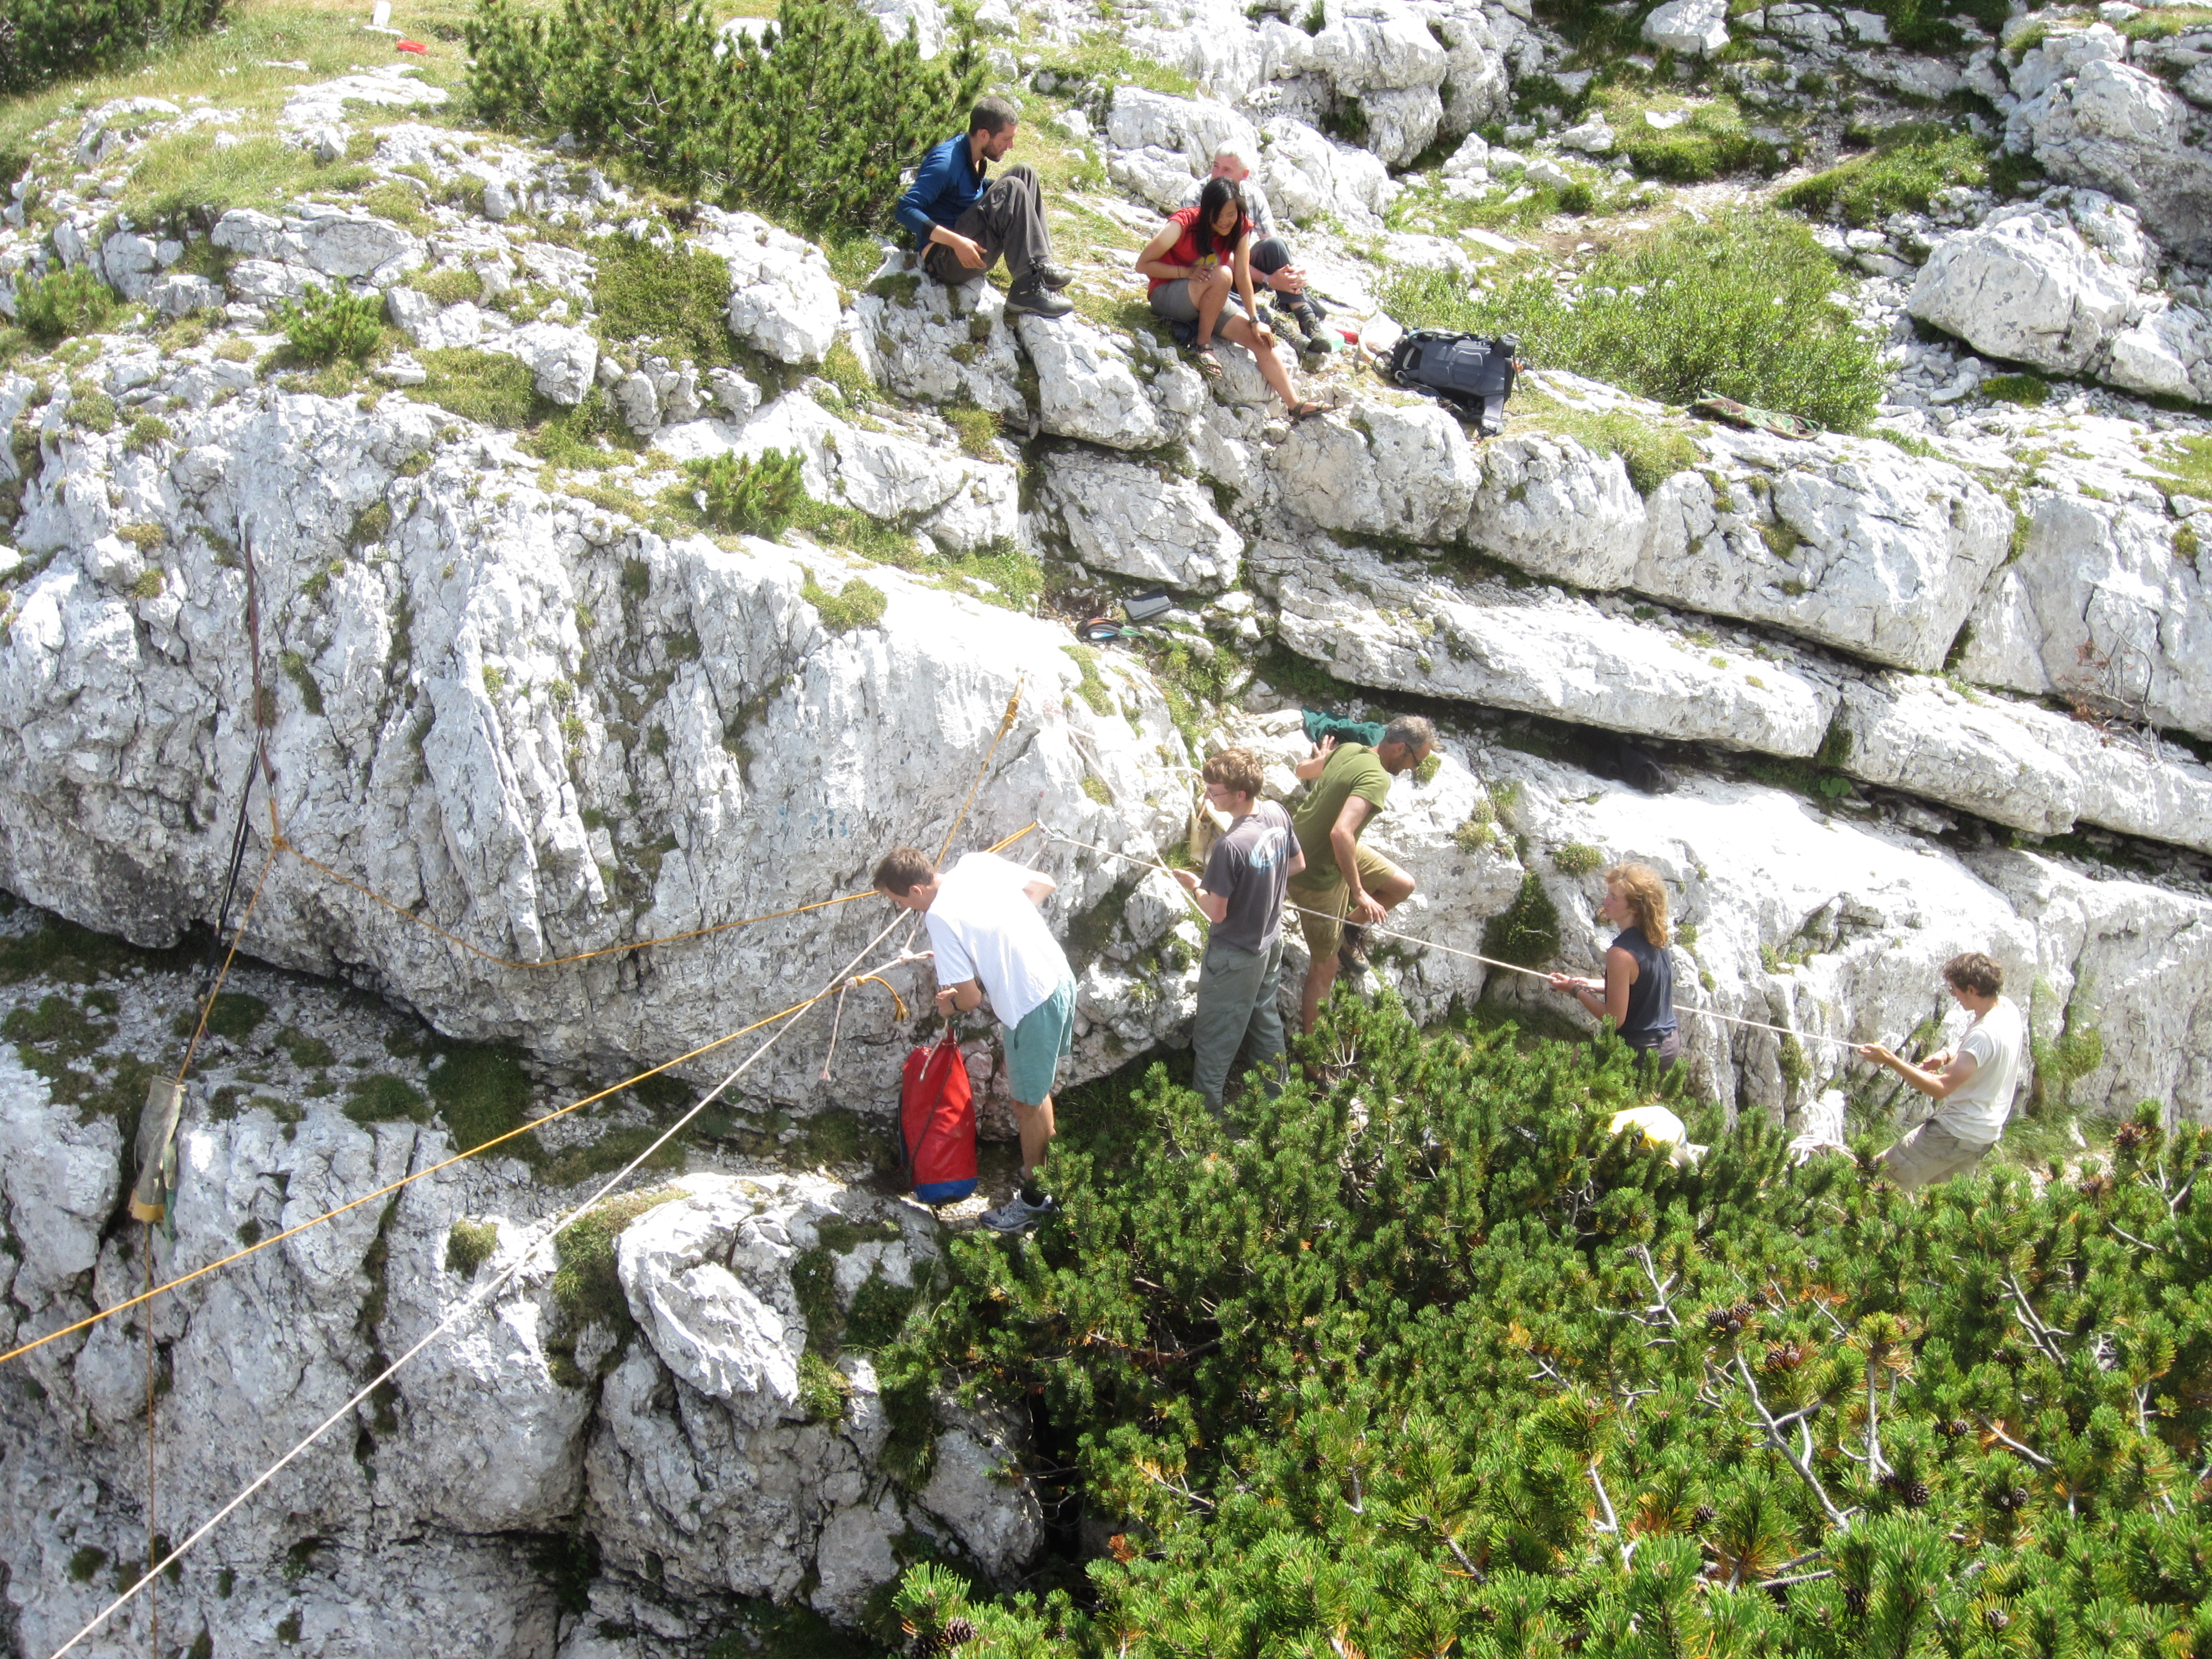
\includegraphics[width = \textwidth]{2012/alex_pitcher/2012-08-10-2334-TharatornSupasiti-IMG_0182--orig.jpg}
\caption{Sam and others haul snow out of the \passage{M10} shakehole to provide drinking water. \pic{Tharatorn Supasiti}} \label{m10 haul}
\end{pagefigure}


\fullwidthbox{Sam's return to Camp \passage{X-Ray}}{

\textit{10/08/12 9:50 pm}

SO happy to be back -- finally. Was apprehensive about coming down after
the adventures of last time -- both coming down and going out turned
into mini epics, but coming down today just took us 2 ½ hours. Compared
to last time's 5 hourish trip down, this felt like such a jolly. The 5
hours were due to an hour stuck at the top of \passage{Skynet} and another hour on
\passage{Zimmer}'s rebelays, but the rebelays posed to[sic] problem today. I was
fully expecting to have to faff with footloops etc to pass the rebelays,
but no such thing was needed. Camp is as homely as I remember. \name{Sam Page}

\textit{11/8/12 11:09 PM}

Surveyed the passage found by Eric \& co. and
pushed some new stuff. Almost 500 m in the book! Named the bolt climb
\passage{Apollo} (as suggested by Gergely), and the horizontal stuff after
that is \passage{Milky Way}. Three main leads in \passage{Milky Way} -- two pitches and one
wide open horizontal virgin passage (!!). [\ldots{}] Now in bed ensconced in TWO nitestars. \name{Clare}

\textit{12/8/12 9:20 AM}

Had a great day yesterday. Clare mentioned that the amount of surveying
we did yesterday may be a record for a virgin surveyor. Hmm\ldots{} data
will reveal all, but it definitely felt like a lot of surveying! Did get
a bit fed up with using the instruments towards the end. But the stuff
we found was very exciting -- and there are existing leads that we left.
Today, we are heading out. Should be ok -- long but it needs
doing\ldots{} \name{Sam}}


\margininbox{Apollo \& Milky Way}{
     \begin{itemize}
    \item Sam Page
    \item Clare Tan
    \end{itemize}}{\explo}

It took me a fairly long time to return to underground camp, but I was immediately glad to be back. Whilst we were heading down to camp, we passed a trio of cavers on their way out. They had found a lot of new horizontal cave passage but had not surveyed this, for valid reasons. Thus, our plan for the next day was to survey this. As my first proper experience of surveying, it was a baptism of fire. According to my partner, it might well be the most surveying done by a first time surveyor, and although it was mostly fairly easy, the novelty did begin to wear off towards the end. This was exciting enough, but we also looked at other passages leading off the main passage, where we were truly the first person to set foot. Even better, the passage that we surveyed eventually continued onto where the connection between the two cave systems was found, meaning that in some small part, I genuinely contributed to the finding of the connection.

\begin{marginfigure}
\checkoddpage \ifoddpage \forcerectofloat \else \forceversofloat \fi
\centering
 \frame{\includegraphics[width=\linewidth]{2012/alex_pitcher/2012-08-10-0618-GergelyAmbrus-IMG_2270--orig.jpg}} 
 \caption{Jonny emerging from \passage{N9}. \pic{Gergely Ambrus}}
 \label{N9 jonny}
\end{marginfigure}

Even though these were my only two deep caving trips, I did do a lot of other caving, including a ‘tourist trip’ down \passage{M16} and a bounce trip partway down to underground camp. Most notably, I was part of a team who went to look at a potential new cave -- \passage{N9} (\passage{Kuk Pot}) -- that had not been properly explored previously beyond the surface. At the end of the day, there were two short pitches rigged that ended in a rift that was too tight to immediately pass, but which definitely continued as the floor below could be seen. More surveying and my first bolting were done that day.

The cumulative effects of my various caving trips meant that I not only became a better caver, but also learnt about exploration caving, bolting, rigging, surveying, assessing caves and route finding – all vitally important if I want to continue caving and one day become more involved in running trips, rather than just following another caver.



\tweet{7:31PM Aug 12, 2012}{Apollo, the climb in Queen's bed chamber, goes to Milky Way, 420m of passage. Vrtnarija now 13462m long.}



I enjoyed my time above ground too. Some days were spent in and around the plateau, including snow hauling, water carrying, cooking, ‘bivvy projects’ or even just recovering from caving. Other days were spent mountain walking, or on other projects such as path cairning. Truthfully, there was not one day that I did not get something out of. Just being up on the mountain, let alone everything else, was fantastic. I grew not only as a caver but as a person: I became fitter, more independent, and more knowledgeable about all sorts of things, like the history of Slovenia and mountain wildlife. Five weeks sounded like a long time before I left, but when I returned home, it seemed to have passed very quickly. I cannot wait to return next year. This year was so successful, in terms of finding new cave and the connection, that I feel a little too lucky to have this success on my first go. But \bignote{there is still so much out there to find}, that, if anything, the future is more exciting and unknown.


\begin{pagefigure}
\checkoddpage \ifoddpage \forcerectofloat \else \forceversofloat \fi
   \centering
\includegraphics[width = \textwidth]{2012/alex_pitcher/2012-08-11-0157-GergelyAmbrus-IMG_2373--orig.jpg}
\caption{One surface project in 2012 was carrying a mountaintop container unit (delivered by helicopter) to its ultimate location within a shakehole near the bivi. \pic{Gergely Ambrus}} \label{container}
\end{pagefigure}

